% Created 2014-10-12 dom 19:59
\documentclass[xcolor={usenames,svgnames,dvipsnames}]{beamer}
\usepackage[utf8]{inputenc}
\usepackage[T1]{fontenc}
\usepackage{fixltx2e}
\usepackage{graphicx}
\usepackage{longtable}
\usepackage{float}
\usepackage{wrapfig}
\usepackage{rotating}
\usepackage[normalem]{ulem}
\usepackage{amsmath}
\usepackage{textcomp}
\usepackage{marvosym}
\usepackage{wasysym}
\usepackage{amssymb}
\usepackage{hyperref}
\tolerance=1000
\usepackage{color}
\usepackage{listings}
\AtBeginSection[]{\begin{frame}[plain]\tableofcontents[currentsection,hideallsubsections]\end{frame}}
\lstset{keywordstyle=\color{blue}, commentstyle=\color{gray!90}, basicstyle=\ttfamily\small, columns=fullflexible, breaklines=true,linewidth=\textwidth, backgroundcolor=\color{gray!23}, basewidth={0.5em,0.4em}, literate={á}{{\'a}}1 {ñ}{{\~n}}1 {é}{{\'e}}1 {ó}{{\'o}}1 {º}{{\textordmasculine}}1}
\usepackage{mathpazo}
\hypersetup{colorlinks=true, linkcolor=Blue, urlcolor=Blue}
\usepackage{fancyvrb}
\DefineVerbatimEnvironment{verbatim}{Verbatim}{boxwidth=\textwidth, fontsize=\tiny, formatcom = {\color{black!70}}}
\usepackage{animate}
\usetheme{Goettingen}
\usecolortheme{rose}
\usefonttheme{serif}
\author{Oscar Perpiñán Lamigueiro}
\date{24 de Octubre de 2014}
\title{Visualización de Series Temporales}
\hypersetup{
  pdfkeywords={},
  pdfsubject={},
  pdfcreator={Emacs 24.3.1 (Org mode 8.2.7c)}}
\begin{document}

\maketitle
\#+begin$_{\text{src}}$ R :exports none  

\section{Introducción}
\label{sec-1}

\lstset{language=R,label= ,caption= ,numbers=none}
\begin{lstlisting}
  ##################################################################
  ## Initial configuration
  ##################################################################
  ## Clone or download the repository and set the working directory
  ## with setwd to the folder where the repository is located.
  
 
  library(lattice)
  library(ggplot2)
  library(latticeExtra)
  library(zoo)
  
  myTheme <- custom.theme.2(pch=19, cex=0.7,
                            region=rev(brewer.pal(9, 'YlOrRd')),
                            symbol = brewer.pal(n=8, name = "Dark2"))
  myTheme$strip.background$col='transparent'
  myTheme$strip.shingle$col='transparent'
  myTheme$strip.border$col='transparent'
  
  xscale.components.custom <- function(...){
      ans <- xscale.components.default(...)
      ans$top=FALSE
      ans}
  yscale.components.custom <- function(...){
      ans <- yscale.components.default(...)
      ans$right=FALSE
      ans}
  myArgs <- list(as.table=TRUE,
                 between=list(x=0.5, y=0.2),
                 xscale.components = xscale.components.custom,
                 yscale.components = yscale.components.custom)
  defaultArgs <- lattice.options()$default.args
  
  lattice.options(default.theme = myTheme,
                  default.args = modifyList(defaultArgs, myArgs))
  ##################################################################
\end{lstlisting}


\subsection{Series temporales}
\label{sec-1-1}
\begin{frame}[label=sec-1-1-1]{Fundamentos básicos}
\end{frame}

\subsection{Paquetes}
\label{sec-1-2}
\begin{frame}[label=sec-1-2-1]{lattice}
\end{frame}
\begin{frame}[label=sec-1-2-2]{ggplot2}
\end{frame}
\begin{frame}[label=sec-1-2-3]{zoo}
\end{frame}

\section{Time Graph of Different Meteorological Variables}
\label{sec-2}

\subsection{Primera aproximación}
\label{sec-2-1}

\begin{frame}[fragile,label=sec-2-1-1]{lattice: \texttt{xyplot}}
 \lstset{language=R,label= ,caption= ,numbers=none}
\begin{lstlisting}
  load('data/aranjuez.RData')
  library(zoo)
  ## The layout argument arranges panels in rows
  xyplot(aranjuez, layout=c(1, ncol(aranjuez)))
\end{lstlisting}

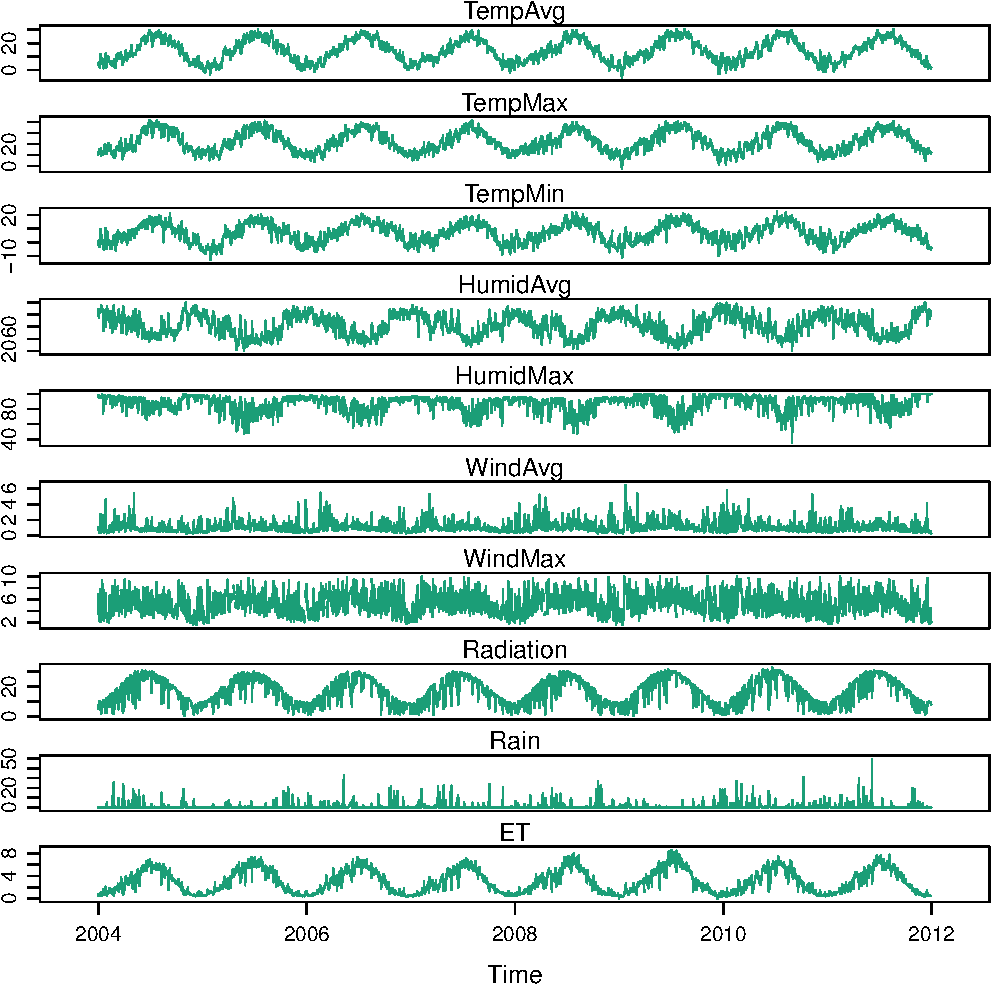
\includegraphics[width=.9\linewidth]{figs/aranjuez.pdf}
\end{frame}

\begin{frame}[fragile,label=sec-2-1-2]{ggplot2: \texttt{autplot}}
 \lstset{language=R,label= ,caption= ,numbers=none}
\begin{lstlisting}
  autoplot(aranjuez) + facet_free()
\end{lstlisting}

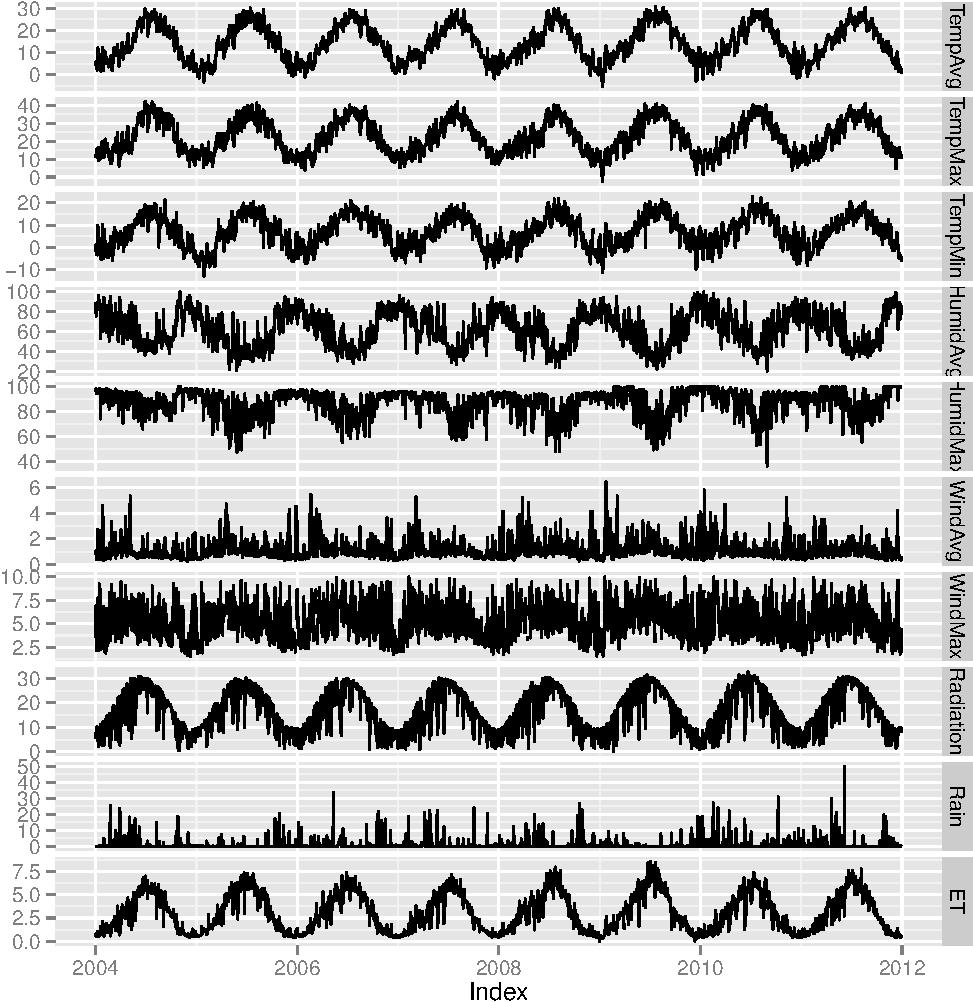
\includegraphics[width=.9\linewidth]{figs/aranjuezGG.pdf}
\end{frame}

\subsection{Anotaciones}
\label{sec-2-2}
\begin{frame}[fragile,label=sec-2-2-1]{lattice}
 \lstset{language=R,label= ,caption= ,numbers=none}
\begin{lstlisting}
  library(grid)
  library(latticeExtra)
  
  ## Auxiliary function to extract the year value of a POSIXct time
  ## index
  Year <- function(x)format(x, "%Y")
  
  xyplot(aranjuez, layout=c(1, ncol(aranjuez)), strip=FALSE,
         scales=list(y=list(cex=0.6, rot=0)),
         panel=function(x, y, ...){
           ## Alternation of years
           panel.xblocks(x, Year,
                         col = c("lightgray", "white"),
                         border = "darkgray")
           ## Values under the average highlighted with red regions
           panel.xblocks(x, y<mean(y, na.rm=TRUE),
                         col = "indianred1",
                         height=unit(0.1, 'npc'))
           ## Time series
           panel.lines(x, y, col='royalblue4', lwd=0.5, ...)
           ## Label of each time series
           panel.text(x[1], min(y, na.rm=TRUE),
                      names(aranjuez)[panel.number()],
                      cex=0.6, adj=c(0, 0), srt=90, ...)
           ## Triangles to point the maxima and minima 
           idxMax <- which.max(y)
           panel.points(x[idxMax], y[idxMax],
                        col='black', fill='lightblue', pch=24)
           idxMin <- which.min(y)
           panel.points(x[idxMin], y[idxMin],
                        col='black', fill='lightblue', pch=25)
         })
\end{lstlisting}
\end{frame}

\begin{frame}[label=sec-2-2-2]{}
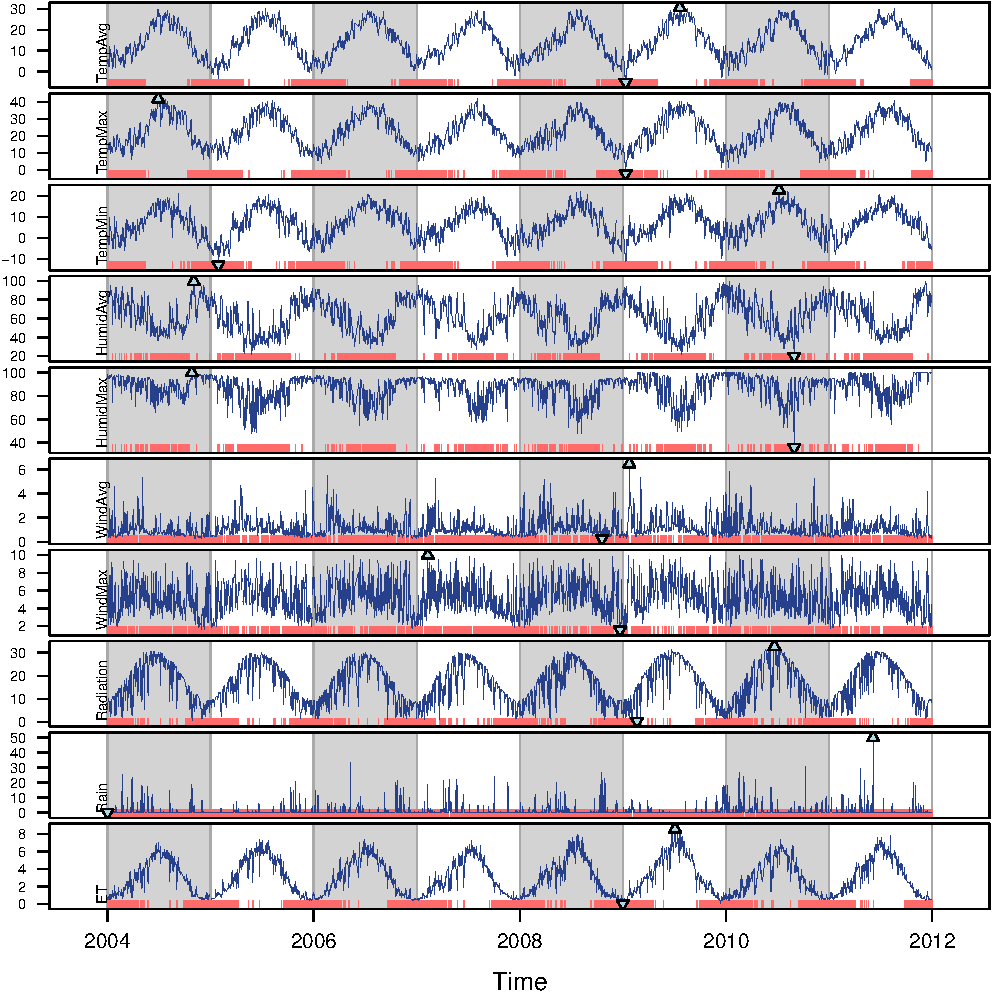
\includegraphics[width=.9\linewidth]{figs/aranjuezXblocks.pdf}
\end{frame}

\begin{frame}[fragile,label=sec-2-2-3]{ggplot2}
 \lstset{language=R,label= ,caption= ,numbers=none}
\begin{lstlisting}
  timeIdx <- index(aranjuez)
  
  long <- fortify(aranjuez, melt=TRUE)
\end{lstlisting}
\end{frame}
\begin{frame}[fragile,label=sec-2-2-4]{The bands of values below the average can be easily extracted with}
 \texttt{scale} because these regions are negative when the \texttt{data.frame} is
centered.
\lstset{language=R,label= ,caption= ,numbers=none}
\begin{lstlisting}
  ## Values below mean are negative after being centered
  scaled <- fortify(scale(aranjuez, scale=FALSE), melt=TRUE)
  ## The 'scaled' column is the result of the centering.
  ## The new 'Value' column store the original values.
  scaled <- transform(scaled, scaled=Value, Value=long$Value)
  underIdx <- which(scaled$scaled <= 0)
  ## 'under' is the subset of values below the average
  under <- scaled[underIdx,]
\end{lstlisting}
\end{frame}

\begin{frame}[fragile,label=sec-2-2-5]{The years bands are defined with the function \texttt{endpoints} from the}
 \texttt{xts} package:

\lstset{language=R,label= ,caption= ,numbers=none}
\begin{lstlisting}
  library(xts)
  ep <- endpoints(timeIdx, on='years')
  N <- length(ep[-1])
  ## 'tsp' is start and 'tep' is the end of each band
  tep <- timeIdx[ep]
  tsp <- timeIdx[ep[-(N+1)]+1]
  ## 'cols' is a vector with the color of each band
  cols <- rep_len(c('gray', 'white'), N)
\end{lstlisting}
\end{frame}
\begin{frame}[fragile,label=sec-2-2-6]{The minima and maxima points of each variable are extracted with}
 \texttt{apply}:
\lstset{language=R,label= ,caption= ,numbers=none}
\begin{lstlisting}
  minIdx <- timeIdx[apply(aranjuez, 2, which.min)]
  minVals <- apply(aranjuez, 2, min, na.rm=TRUE)
  mins <- data.frame(Index=minIdx,
                     Value=minVals,
                     Series=names(aranjuez))
  
  maxIdx <- timeIdx[apply(aranjuez, 2, which.max)]
  maxVals <- apply(aranjuez, 2, max, na.rm=TRUE)
  maxs <- data.frame(Index=maxIdx,
                     Value=maxVals,
                     Series=names(aranjuez))
\end{lstlisting}
\end{frame}

\begin{frame}[fragile,label=sec-2-2-7]{With \texttt{ggplot} we define the canvas, and the layers of information are}
 added successively:
\lstset{language=R,label= ,caption= ,numbers=none}
\begin{lstlisting}
  ggplot(data=long, aes(Index, Value)) +
      ## Time series of each variable
      geom_line(colour = "royalblue4", lwd = 0.5) +
      ## Year bands
      annotate(geom='rect', ymin = -Inf, ymax = Inf,
                xmin=tsp, xmax=tep,
                fill = cols, alpha = 0.4) +
      ## Values below average
      geom_rug(data=under,
               sides='b', col='indianred1') +
      ## Minima
      geom_point(data=mins, pch=25) +
      ## Maxima
      geom_point(data=maxs, pch=24) +
      ## Axis labels and theme definition
      labs(x='Time', y=NULL) +
      theme_bw() +
      ## Each series is displayed in a different panel with an
      ## independent y scale
      facet_free()
\end{lstlisting}
\end{frame}


\section{Time Series of Variables with the Same Scale}
\label{sec-3}

\subsection{Primera aproximación}
\label{sec-3-1}
\begin{frame}[fragile,label=sec-3-1-1]{lattice xyplot}
 \lstset{language=R,label= ,caption= ,numbers=none}
\begin{lstlisting}
  load('data/navarra.RData')
\end{lstlisting}

\lstset{language=R,label= ,caption= ,numbers=none}
\begin{lstlisting}
  avRad <- zoo(rowMeans(navarra, na.rm=1), index(navarra))
  pNavarra <- xyplot(navarra - avRad,
                     superpose=TRUE, auto.key=FALSE,
                     lwd=0.5, alpha=0.3, col='midnightblue') 
  pNavarra
\end{lstlisting}
\end{frame}

\begin{frame}[label=sec-3-1-2]{}
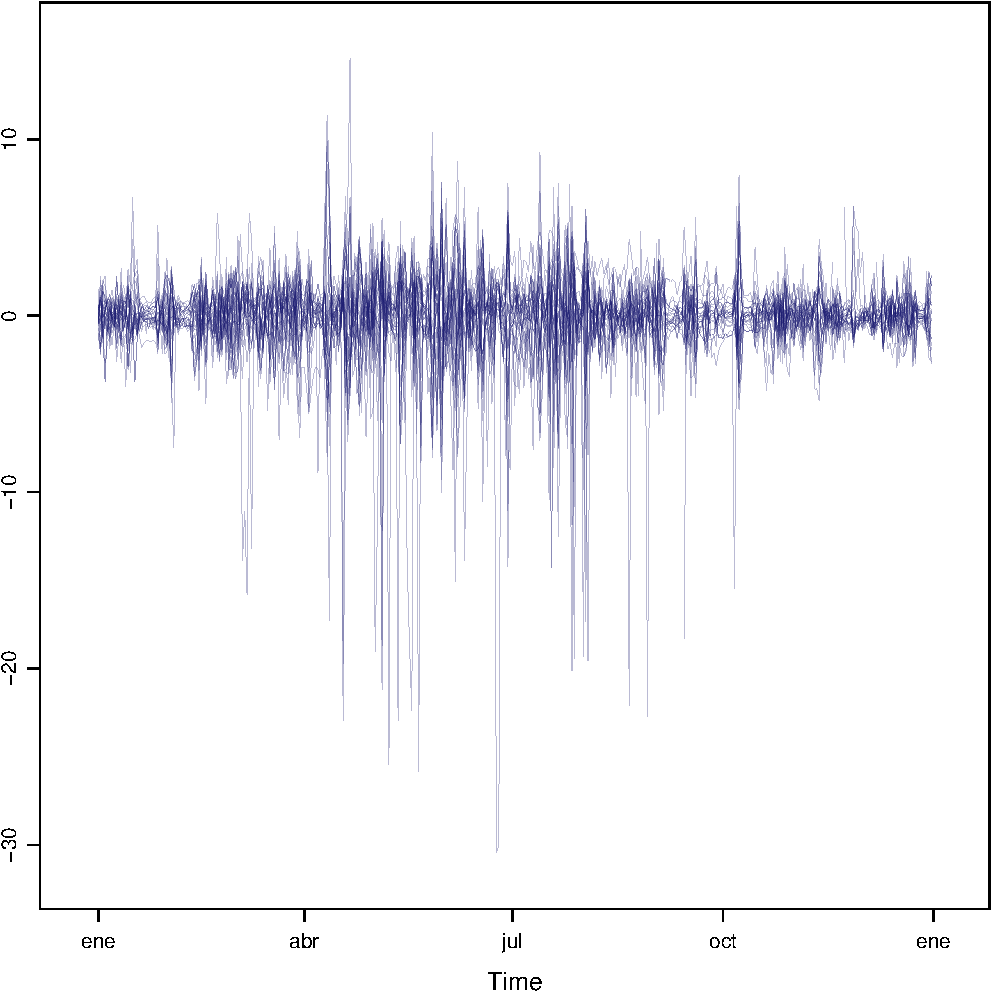
\includegraphics[width=.9\linewidth]{figs/navarra.pdf}
\end{frame}

\subsection{Aspect Ratio and Rate of Change}
\label{sec-3-2}

\begin{frame}[fragile,label=sec-3-2-1]{lattice}
 \lstset{language=R,label= ,caption= ,numbers=none}
\begin{lstlisting}
  xyplot(navarra - avRad,
         aspect='xy', cut=list(n=3, overlap=0.1),
         strip=FALSE,
         superpose=TRUE, auto.key=FALSE,
         lwd=0.5, alpha=0.3, col='midnightblue')
\end{lstlisting}
\end{frame}

\begin{frame}[label=sec-3-2-2]{}
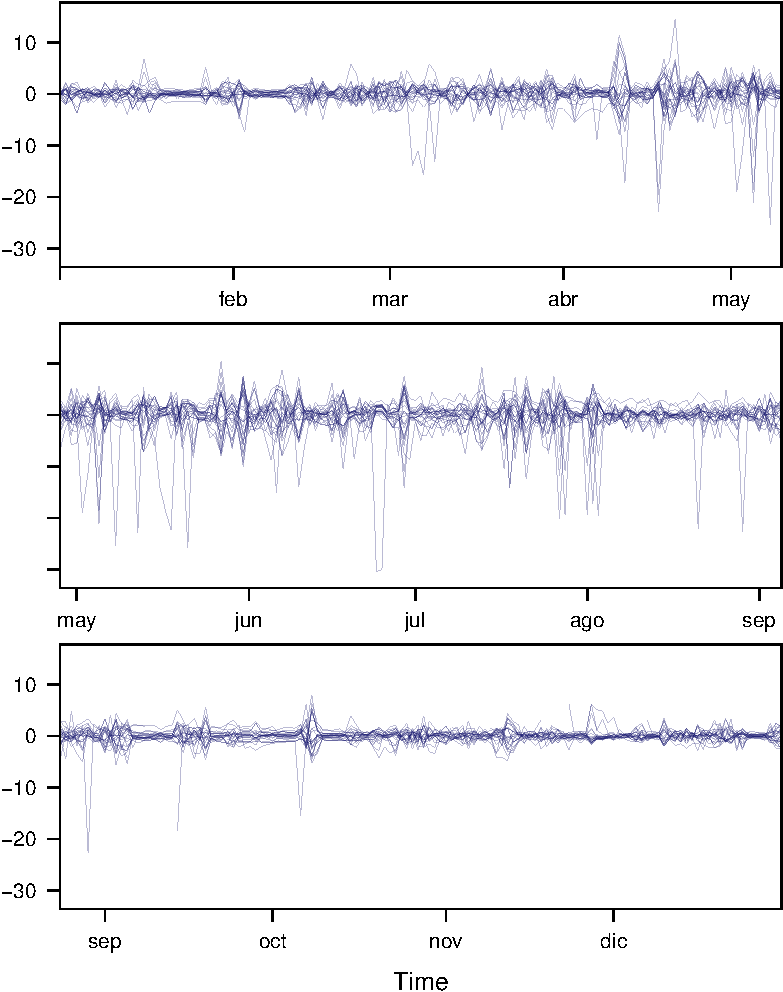
\includegraphics[width=.9\linewidth]{figs/navarraBanking.pdf}
\end{frame}


\subsection{The Horizon Graph}
\label{sec-3-3}

\begin{frame}[fragile,label=sec-3-3-1]{horizonplot}
 \lstset{language=R,label= ,caption= ,numbers=none}
\begin{lstlisting}
  library(latticeExtra)
  
  horizonplot(navarra-avRad,
              layout=c(1, ncol(navarra)),
              origin=0, colorkey=TRUE)
\end{lstlisting}
\end{frame}

\begin{frame}[label=sec-3-3-2]{}
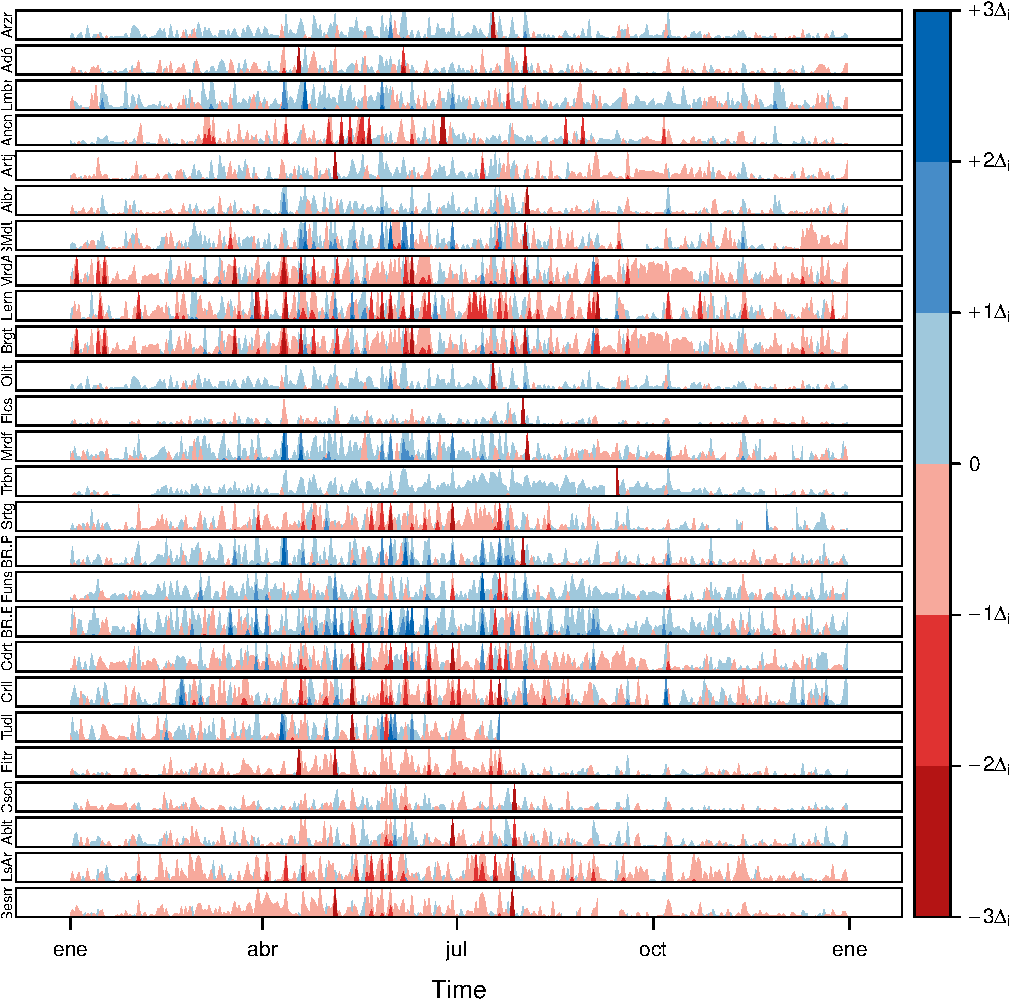
\includegraphics[width=.9\linewidth]{figs/navarraHorizonplot.pdf}
\end{frame}

\begin{frame}[fragile,label=sec-3-3-3]{Diferencias}
 \lstset{language=R,label= ,caption= ,numbers=none}
\begin{lstlisting}
  Ta <- aranjuez$TempAvg
  timeIndex <- index(aranjuez)
  longTa <- ave(Ta, format(timeIndex, '%j'))
  diffTa <- (Ta - longTa)
\end{lstlisting}


\lstset{language=R,label= ,caption= ,numbers=none}
\begin{lstlisting}
  years <- unique(format(timeIndex, '%Y'))
  
  horizonplot(diffTa, cut=list(n=8, overlap=0),
              colorkey=TRUE, layout=c(1, 8),
              scales=list(draw=FALSE, y=list(relation='same')),
              origin=0, strip.left=FALSE) +
      layer(grid.text(years[panel.number()], x = 0, y = 0.1, 
                      gp=gpar(cex=0.8),
                      just = "left"))
\end{lstlisting}
\end{frame}

\begin{frame}[label=sec-3-3-4]{}
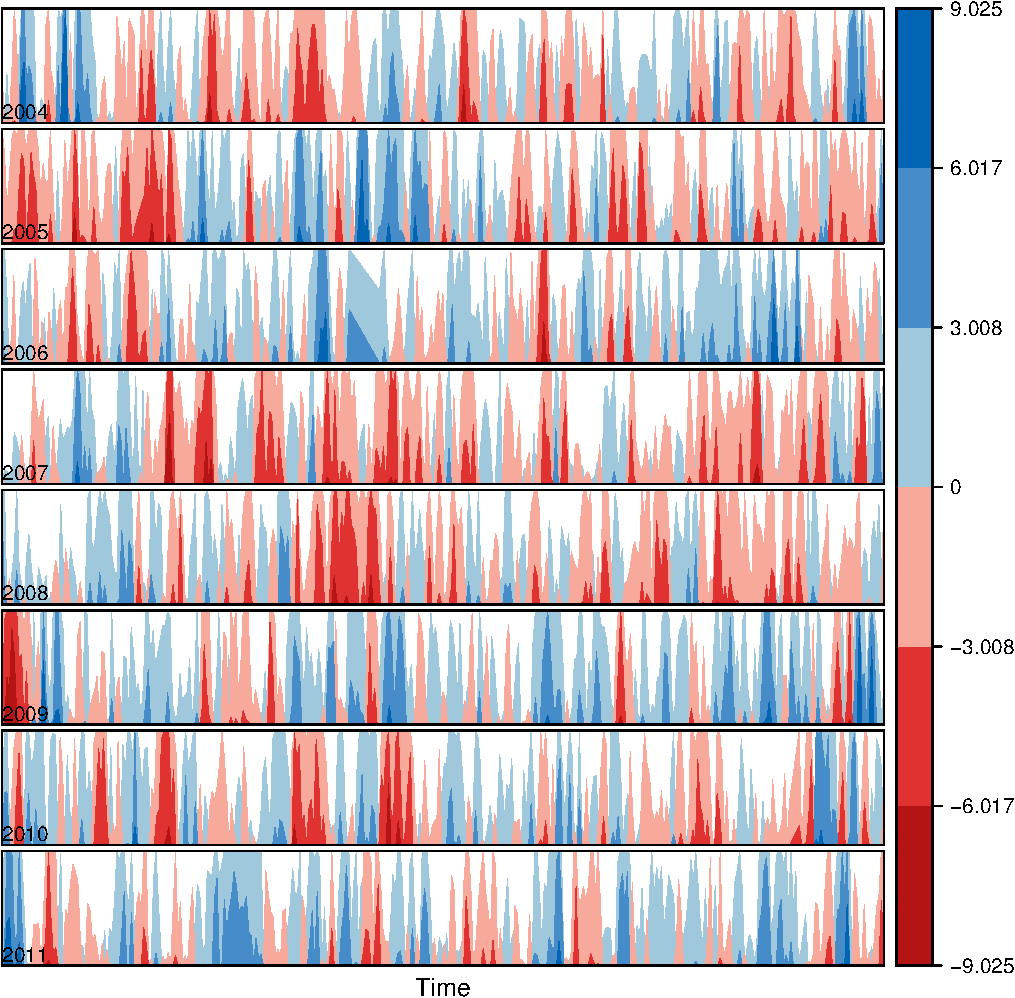
\includegraphics[width=.9\linewidth]{figs/diffTa_horizon.pdf}
\end{frame}


\section{Scatterplot Matrix: Time as a Grouping Variable}
\label{sec-4}

\subsection{Introducción}
\label{sec-4-1}

\begin{frame}[label=sec-4-1-1]{Que es}
\end{frame}

\subsection{Realización}
\label{sec-4-2}

\begin{frame}[fragile,label=sec-4-2-1]{lattice}
 \lstset{language=R,label= ,caption= ,numbers=none}
\begin{lstlisting}
  load('data/aranjuez.RData')
  
  ## Red-Blue palette with black added (12 colors)
  colors <- c(brewer.pal(n=11, 'RdBu'), '#000000')
  ## Rearrange according to months (darkest for summer)
  colors <- colors[c(6:1, 12:7)]
  
  splom(~as.data.frame(aranjuez),
          groups=format(index(aranjuez), '%m'),
        auto.key=list(space='right', 
            title='Month', cex.title=1),
        pscale=0, varname.cex=0.7, xlab='',
          par.settings=custom.theme(symbol=colors,
              pch=19), cex=0.3, alpha=0.1)
\end{lstlisting}


\includegraphics[width=.9\linewidth]{figs/aranjuezSplom.png}
\end{frame}



\subsection{Hexagonal Binning}
\label{sec-4-3}

\begin{frame}[fragile,label=sec-4-3-1]{Código}
 \lstset{language=R,label= ,caption= ,numbers=none}
\begin{lstlisting}
  library(hexbin)
  
  splom(~as.data.frame(aranjuez),
             panel=panel.hexbinplot, xlab='',
             colramp=BTC,
             diag.panel = function(x, ...){
               yrng <- current.panel.limits()$ylim
               d <- density(x, na.rm=TRUE)
               d$y <- with(d, yrng[1] + 0.95 * diff(yrng) * y / max(y))
               panel.lines(d)
               diag.panel.splom(x, ...)
             },
             lower.panel = function(x, y, ...){
               panel.hexbinplot(x, y, ...)
               panel.loess(x, y, ..., col = 'red')
             },
             pscale=0, varname.cex=0.7
             )
\end{lstlisting}
\end{frame}

\begin{frame}[label=sec-4-3-2]{}
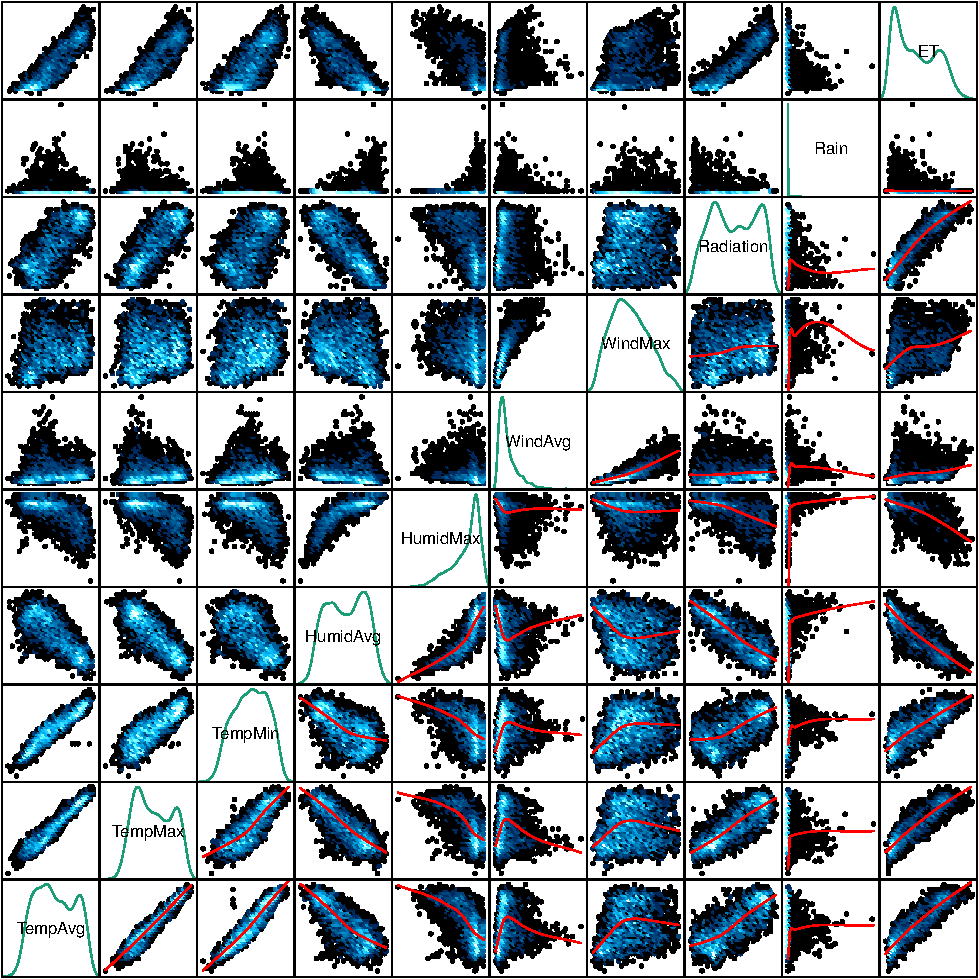
\includegraphics[width=.9\linewidth]{figs/aranjuezSplomHexbin.pdf}
\end{frame}

\section{Scatterplot with Time as a Conditioning Variable}
\label{sec-5}

\subsection{Introducción}
\label{sec-5-1}

\begin{frame}[label=sec-5-1-1]{Introducción}
\end{frame}

\subsection{Código}
\label{sec-5-2}

\begin{frame}[fragile,label=sec-5-2-1]{ggplot2}
 \lstset{language=R,label= ,caption= ,numbers=none}
\begin{lstlisting}
  ggplot(data=aranjuezRshp, aes(Radiation, Temperature)) +
      facet_grid(Statistic ~ month) +
      geom_point(col='skyblue4', pch=19, cex=0.5, alpha=0.3) +
      geom_rug() +
      stat_smooth(se=FALSE, method='loess', col='indianred1', lwd=1.2) +
      theme_bw()
\end{lstlisting}
\end{frame}

\begin{frame}[label=sec-5-2-2]{}
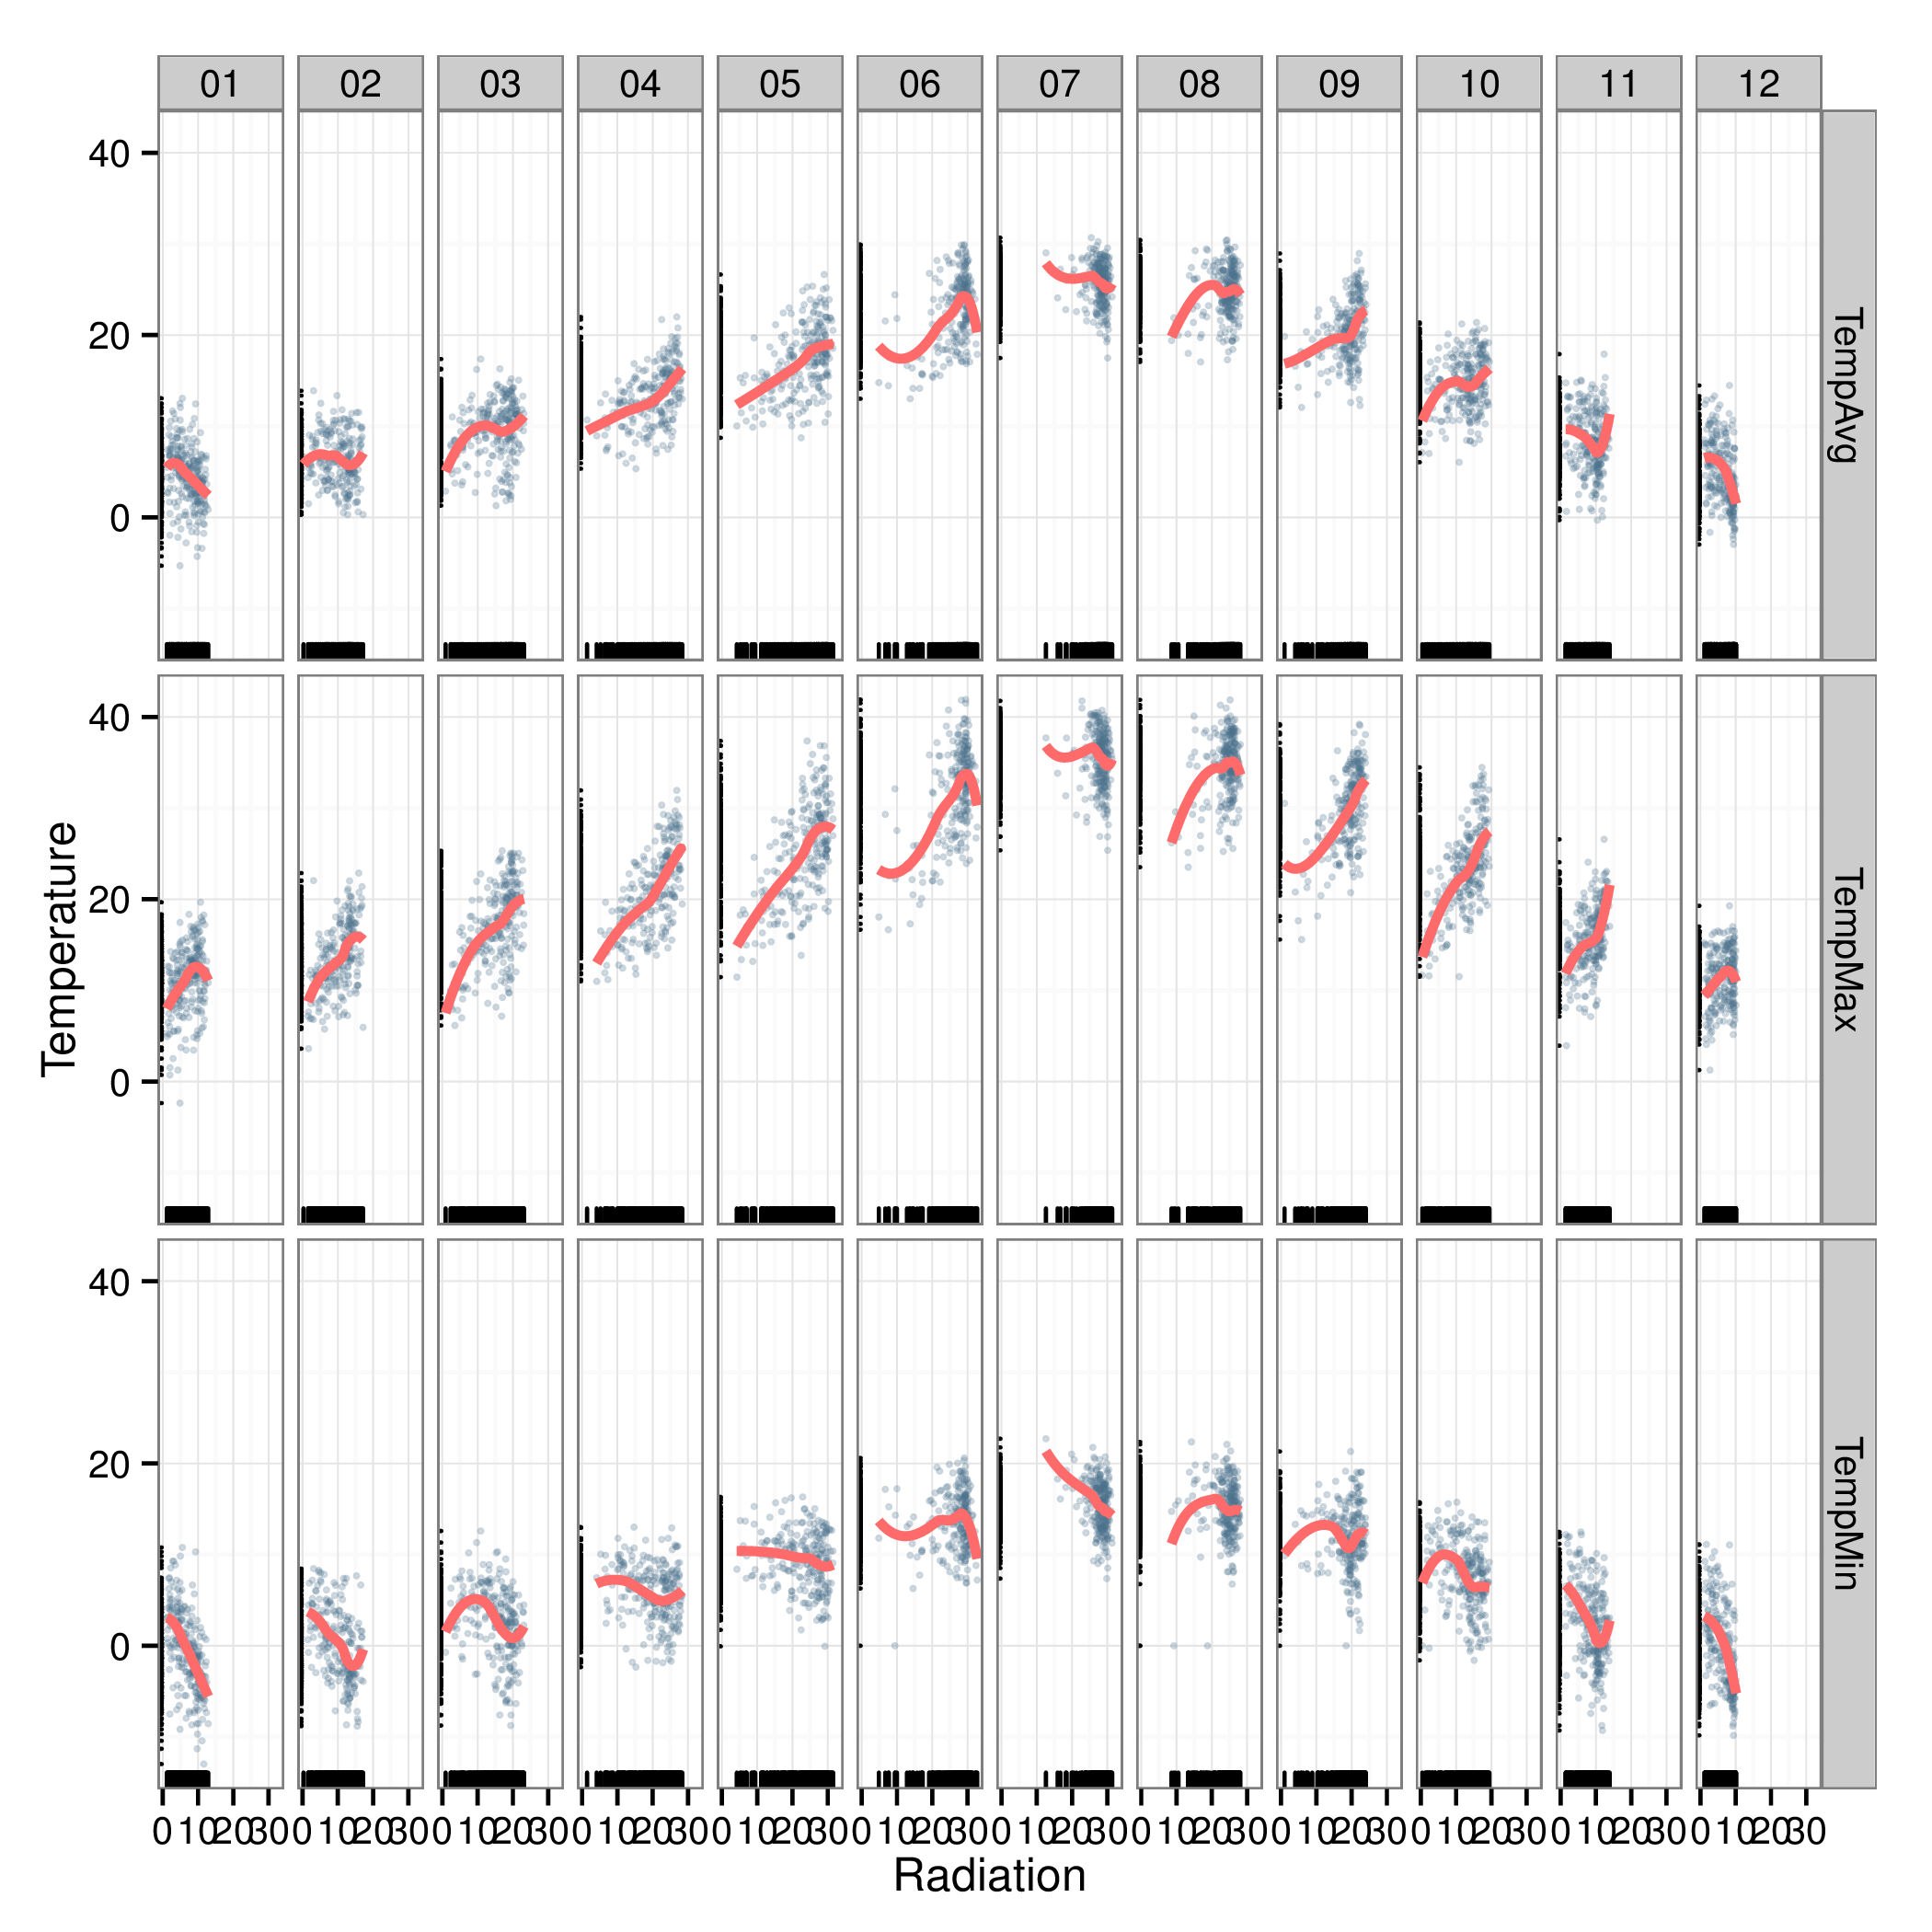
\includegraphics[width=.9\linewidth]{figs/aranjuezFacetGrid.png}
\end{frame}


\begin{frame}[fragile,label=sec-5-2-3]{lattice}
 \lstset{language=R,label= ,caption= ,numbers=none}
\begin{lstlisting}
  useOuterStrips(xyplot(Temperature ~ Radiation | month * Statistic,
                        data=aranjuezRshp,
                        between=list(x=0),
                        col='skyblue4', pch=19,
                        cex=0.5, alpha=0.3)) +
      layer({
          panel.rug(..., col.line='indianred1', end=0.05, alpha=0.6)
          panel.loess(..., col='indianred1', lwd=1.5, alpha=1)
      })
\end{lstlisting}
\end{frame}


\begin{frame}[label=sec-5-2-4]{}
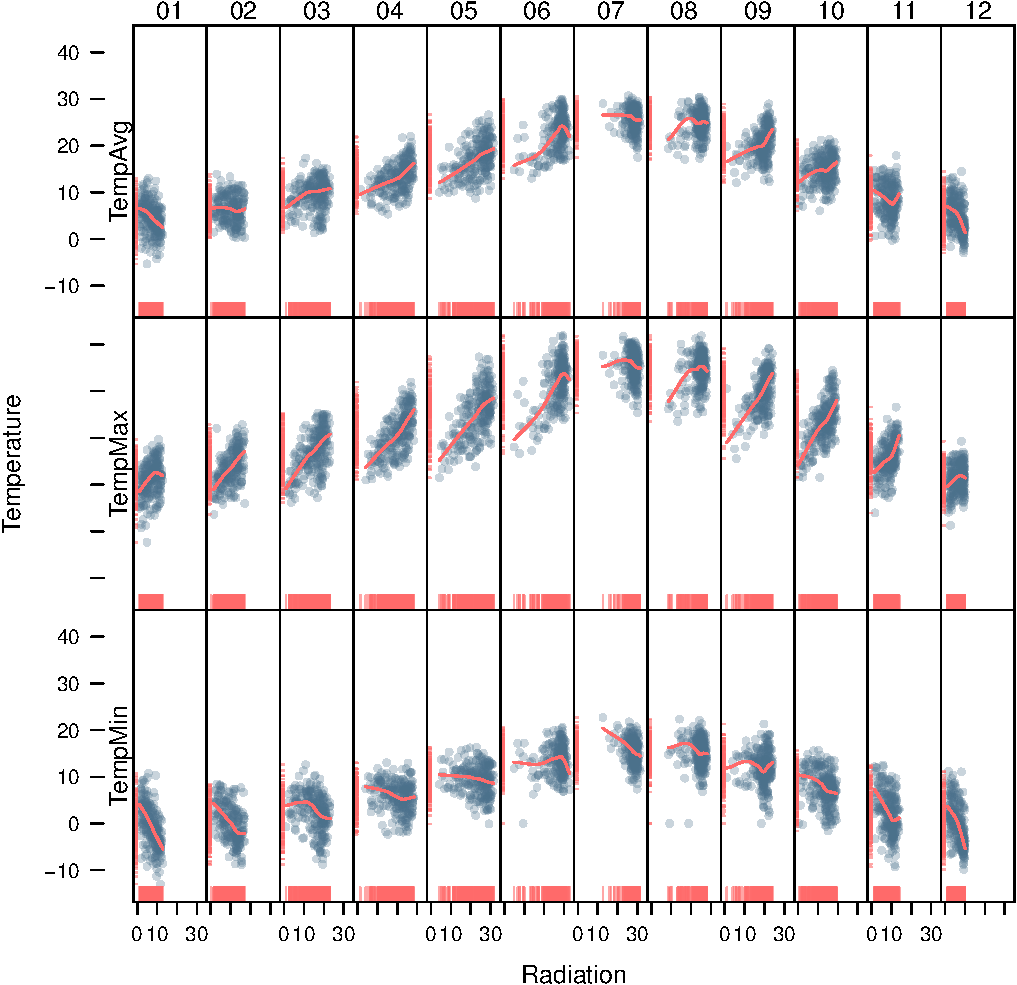
\includegraphics[width=.9\linewidth]{figs/aranjuezOuterStrips.pdf}
\end{frame}


\subsection{}
\label{sec-5-3}
% Emacs 24.3.1 (Org mode 8.2.7c)
\end{document}